\documentclass[11pt]{article}
\usepackage{amsmath} % Math
\usepackage{amssymb} % Math symbols
\usepackage[english]{babel} % Language
\usepackage{fancyhdr} % Header
\usepackage[a4paper, total={15cm, 20cm}]{geometry} % Dimensions of the paper and the text area
\usepackage[utf8]{inputenc} % encoding in UTF, needed for umlauts if German
\usepackage{mathtools} % Text above arrows
\usepackage{msc} % Drawing MSCs
\usepackage{multicol} % Multiple columns
\usepackage[explicit]{titlesec} % Automatic section titles
\usepackage{tikz} % Diagrams
\usetikzlibrary{arrows.meta, automata, shapes, matrix,positioning}
\usepackage{enumitem}   % Enumeration item
\usepackage{float}
\usepackage{verbatim}


% Other packages that might be useful in the future
%\usepackage{lingmacros}
%\usepackage{tree-dvips}
%\usepackage{ulem}
%\usepackage{amsthm}
%\usepackage{amsbsy}
%\usepackage{textcomp,gensymb}
%\usepackage{graphicx}
%\usepackage{mathtools}

% Custom variant of msc environment:
% - No "msc" keyword, longer partial messages
% - Increased vertical distance between messages
% - Less distance to the frame left and right
% - Less distance between header and processes
% - Less distance between footer and frame
% - Passing all given options down to the msc environment
\newenvironment{cmsc}[1][]{\msc[msc keyword={}, self message width=1.1cm, level height=0.6cm, environment distance=1.2cm, head top distance=0.75cm, foot distance=0.5cm, #1]}{\endmsc}

% No indentation at new paragraphs
\setlength{\parindent}{0pt}

% Distance between columns
\setlength{\columnsep}{1cm}
% Vertical line between columns
\setlength{\columnseprule}{0.5pt}
\def\columnseprulecolor{\color{gray}}

% Settings
\newcommand{\sheetNr}{2}
\newcommand{\red}[1]{\color{red}#1\color{black}}

%% Header
\fancyhf{}
\pagestyle{fancy}
\lhead{Model Checking Exercise Sheet \sheetNr}
\rhead{Aaron Grabowy: 345766\\ Timo Bergerbusch: 344408\\ Felix Linhart: 318801}
\setlength{\headheight}{40pt}

%% Automatic section titles
\titleformat{\section}{\normalfont\Large\bfseries}{}{0em}{Exercise #1}
\titleformat{\subsection}{\normalfont\large\bfseries}{}{0em}{#1)}

\begin{document}
	
	\section{1}
	\subsection{a}
	
	Let $TS_1, TS_2$ and $TS_3$ be:\\
	\vspace{-4em}
	\begin{figure}[H]
		\centering
		\begin{tikzpicture}[shorten >=1pt,node distance=2cm,on grid,auto] 
		\node[state,initial, initial text = ] (t10) {$t_0$};
		\node[state] (t11) [right = of t10] {$t_1$};
		
		\path[->] (t10) edge node {$\alpha$} (t11);
		\end{tikzpicture}
	\end{figure}
	Further let $H = \emptyset$ and $H'=\{\alpha\}$. A node contains the shorthand notation of for example ``0 0'' to denote that $TS_1$ and $TS_2$ (in the second case $TS_2$ and $TS_3$) are in state $t_0$. Analogously for ``0 0 0'' and $TS_1,TS_2$ and $TS_3$. Then we can construct $TS_4 \coloneqq (TS_1 ||_{H} TS_2) ||_{H'} TS_3$ as:\\
	
	\begin{figure}[H]
		\begin{tikzpicture}[shorten >=1pt,node distance=2cm,on grid,auto] 
		% left 
		\node[state, initial, initial text = ] (00) {0 0};
		\node[state, below left = of 00] (01) {0 1};
		\node[state, below right = of 00] (10) {1 0};
		\node[state, below right = of 01] (11) {1 1};
		\node[right = of 10] (add) {$||_{H'} TS_3$};
		
		% arrow
		\node[right = of add] (arrow) {$\Rightarrow$};
		
		% right
		\node[state, initial, initial text = , right = 9cm of 00] (000) {0 0 0};
		\node[state, below left = 3cm of 000] (011) {0 1 1};
		\node[state, below right = 3cm of 000] (101) {1 0 1};
		
		%left 
		\path[->] (00) edge node {$\alpha$} (01)
		(00) edge node {$\alpha$} (10)
		(10) edge node {$\alpha$} (11)
		(01) edge node {$\alpha$} (11);
		
		% right
		\path[->] (000) edge node {$\alpha$} (011)
		(000) edge node {$\alpha$} (101);
		\end{tikzpicture}
	\end{figure}
	
	Now we construct $TS_4' \coloneqq TS_1 ||_H (TS_2 ||_{H'} TS_3)$:
	\begin{figure}[H]
		\begin{tikzpicture}[shorten >=1pt,node distance=2cm,on grid,auto] 
		% left 
		\node[state, initial, initial text = ] (00) {0 0};
		\node[state, right = of 00] (11) {1 1};
		\node[left = of 00] (add) {$TS_1 ||_H$};
		
		% arrow
		\node[right = of 11] (arrow) {$\Rightarrow$};
		
		% right
		\node[state, initial, initial text = , above right = 1.5cm and 8cm of 00] (000) {0 0 0};
		\node[state, below right = of 000] (100) {1 0 0};
		\node[state, below left = of 000] (011) {0 1 1};
		\node[state, below right = of 011] (111) {1 1 1};
		
		%left 
		\path[->] (00) edge node {$\alpha$} (11);
		
		% right
		\path[->] (000) edge node {$\alpha$} (100)
		(000) edge node {$\alpha$} (011)
		(100) edge node {$\alpha$} (111)
		(011) edge node {$\alpha$} (111);
		\end{tikzpicture}
	\end{figure}
	
	As we can see $TS_4 \neq TS_4'$ and therefore in general the handshaking $||_H$ is not associative.
	
	\subsection{b}
	
	In order two proof that the bijection $f_\approx$  preserves the stated transition relation, we consider 3 base cases:
	\subsubsection*{i) $\alpha \in Act_1 \setminus (Act_2 \cup Act_3)$} \label{i}
	If $\alpha$ is neither contained in $Act_2$ nor $Act_3$ then for every state $\langle \langle s_1 , s_2 \rangle s_3 \rangle$ and every transition $(s_1,\alpha, s_1')\in \rightarrow_1$ there exists a transition 
	$$(\langle \langle s_1 , s_2 \rangle, s_3 \rangle,\alpha, \langle \langle s_1' , s_2 \rangle, s_3 \rangle)\in \rightarrow_L$$
	Since $\alpha\notin Act_2\cup Act_3$ the respective states do not change. The handshaking of $TS_2$ and $TS_3$ does not have any impact on the usage of $\alpha$. So there are also the transitions
	$$(\langle s_1 , \langle s_2 , s_3 \rangle \rangle,\alpha, \langle s_1' , \langle s_2 , s_3 \rangle \rangle)\in \rightarrow_R$$ 
	$$\Leftrightarrow(f_\approx(\langle \langle s_1 , s_2 \rangle, s_3 \rangle),\alpha, f_\approx(\langle \langle s_1' , s_2 \rangle, s_3 \rangle))\in \rightarrow_R$$
	
	\subsubsection*{ii) $\alpha \in (Act_1 \cap Act_2) \setminus Act_3$}
	$\alpha \notin Act_3$ means, that we have to distinguish three further cases based on the current state $\langle \langle s_1 , s_2 \rangle s_3 \rangle$:
	\begin{enumerate}
		\item $(s_1,\alpha, s_1')\in \rightarrow_1$ and $(s_2,\alpha, s_2')\in \rightarrow_2$:\\
		Since both current states $s_1$ and $s_2$ have an available $\alpha$ transition the handshaking of these two would create a state $\langle s_1, s_2 \rangle \xrightarrow{\alpha} \langle s_1', s_2' \rangle$. Since $\alpha \notin Act_3$ the handshaking with $TS_3$ then only creates a crossproduct of all such $\langle s_1, s_2 \rangle$ states with some state $s_3\in S_3$. This would infer that
		$$ (\langle \langle s_1 , s_2 \rangle s_3 \rangle, \alpha, \langle \langle s_1' , s_2' \rangle s_3 \rangle) \in \rightarrow_L$$
		
		If we first compute the handshaking $TS_2 || TS_3$ we would get states, where all transitions using $\alpha$ only change the state of $TS_2$. Performing the second handshake would synchronize the transitioning of $TS_1$ and $TS_2$ using $\alpha$ while still not changing $s_3$. So we get
		$$(\langle s_1 , \langle s_2 , s_3 \rangle \rangle,\alpha, \langle s_1' , \langle s_2' , s_3 \rangle \rangle)\in \rightarrow_R$$
		$$\Leftrightarrow(f_\approx(\langle \langle s_1 , s_2 \rangle, s_3 \rangle),\alpha, f_\approx(\langle \langle s_1' , s_2' \rangle, s_3 \rangle))\in \rightarrow_R$$
		
		\item $(s_1,\alpha, s_1')\in \rightarrow_1$ and $(s_2,\alpha, s_2')\notin \rightarrow_2$:\\
		This would infer that we can not use any transition containing $\alpha$, since both $TS_1$ and $TS_2$ would need to use an $\alpha$ transition. Since $TS_2$, which is in state $s_2$ has no possible transition for $\alpha$, $TS_1$ is not allowed to move.\\
		So for such a state $\langle s_1, s_2 \rangle \in (TS_1 || TS_2)$ there exists no $\alpha$ transition. Also synchronising over $TS_3$ does not change anything about the $\alpha$ transitions. Therefore
		$$(\langle \langle s_1 , s_2 \rangle s_3 \rangle, \alpha, \langle \langle s_1' , s_2' \rangle s_3 \rangle) \notin \rightarrow_L$$
		
		In order to fulfil the condition we now show that also the right side does not have such a transition.\\
		
		Performing the handshake of $TS_2||TS_3$ would create the states $\langle s_2, s_3 \rangle$. Since per assumption $s_2$ does not have a $\alpha$ transition also $\langle s_2, s_3 \rangle$ does not have one. Now also synchronising $TS_1$ can not add a $\alpha$ transition, since it would have to synchronise with $TS_2$ and therefore $s_2$ must have an $\alpha$ transition. This is not the case. So 
		$$(\langle s_1 , \langle s_2 , s_3 \rangle \rangle,\alpha, \langle s_1' , \langle s_2' , s_3 \rangle \rangle)\notin \rightarrow_R$$
		$$\Leftrightarrow(f_\approx(\langle \langle s_1 , s_2 \rangle, s_3 \rangle),\alpha, f_\approx(\langle \langle s_1' , s_2' \rangle, s_3 \rangle))\notin \rightarrow_R$$
		
		
		\item $(s_1,\alpha, s_1')\notin \rightarrow_1$ and $(s_2,\alpha, s_2')\in \rightarrow_2$:\\
		This case is completely analogue to the second case.
		
	\end{enumerate}
	
	\subsubsection*{iii) $\alpha \in Act_1 \cap Act_2 \cap Act_3$}
	\begin{enumerate}
		\item  $(s_1,\alpha, s_1')\in \rightarrow_1$ and $(s_2,\alpha, s_2')\in \rightarrow_2$ and $(s_3, \alpha, s_3')$:\\
		First performing the $TS_1 ||TS_2$ handshake we receive states $\langle s_1, s_2 \rangle$ with $\langle s_1, s_2 \rangle \xrightarrow{\alpha} \langle s_1', s_2' \rangle$. Afterwards synchronizing with $TS_3$ means that every such mentioned state would also change $s_3$ to $s_3'$, since they synchronize over $\alpha$. So:
		$$ (\langle \langle s_1 , s_2 \rangle s_3 \rangle, \alpha, \langle \langle s_1' , s_2' \rangle s_3' \rangle) \in \rightarrow_L$$
		Completely analogously we can first compute $TS_2||TS_3$ and then $TS_1 || (TS_2 || TS_3)$. This will yield the same result and thus:
		$$(\langle s_1 , \langle s_2 , s_3 \rangle \rangle,\alpha, \langle s_1' , \langle s_2' , s_3' \rangle \rangle)\in \rightarrow_R$$
		$$\Leftrightarrow(f_\approx(\langle \langle s_1 , s_2 \rangle, s_3 \rangle),\alpha, f_\approx(\langle \langle s_1' , s_2' \rangle, s_3' \rangle))\in \rightarrow_R$$
		\item If any state $s_i \in \{s_1, s_2, s_3\}$ does not have an $\alpha$ transition we can, analogously to case ii.2) deduce, that there can not be an $\alpha$ transition for such a state $\langle \langle s_1, s_2 \rangle s_3 \rangle$ in $\rightarrow_L$ since this would need all $s_i$'s to have an $\alpha$ transition.\\
		Also we can directly infer that the same holds for $f_\approx (\langle \langle s_1, s_2 \rangle s_3 \rangle) = \langle s_1 \langle s_2 , s_3 \rangle \rangle$ for the exact same reason.
	\end{enumerate}
	
	This finally concludes in 
	$$l) \xrightarrow{\alpha}_L (l') \Rightarrow f_\approx (l) \xrightarrow{\alpha}_R (l')$$
	\subsection{c}
	First we build $TS_4\coloneqq TS_1 || TS_2$:\\
	\begin{figure}[H]
		\centering
		\begin{tikzpicture}[shorten >=1pt,node distance=3cm,on grid,auto] 
		\node[state, initial, initial text = ] (15) {1,5};
		\node[state, above = of 15] (17) {1,7};
		
		\node[state, right = of 17] (37) {3,7};
		\node[state, above = of 37] (27) {2,7};
		\node[state, right = of 27] (47) {4,7};
		
		\node[state, right = of 15] (35) {3,5};
		\node[state, below = of 35] (26) {2,6};
		\node[state, right = of 26] (46) {4,6};
		%	\node[state, right = of 46] (45) {4,5};
		
		\path[->] (15) edge[bend left = 20] node {$\alpha$} (26)
		(15) edge                 node {$\beta$}  (35)
		(17) edge[bend left = 20] node {$\alpha$} (27)
		(27) edge[bend left = 20] node {$\alpha$} (17)
		(17) edge node {$\beta$}  (37)
		(37) edge                 node {$\alpha$} (47)
		(27) edge[bend left = 20] node {$\beta$}  (47)
		(47) edge[bend left = 20] node {$\beta$}  (27)
		(35) edge                 node {$\alpha$} (46)
		(26) edge[bend left = 20] node {$\beta$}  (46)
		(46) edge[bend left = 20] node {$\beta$}  (26)
		%			  (46) edge[bend left = 20] node {$\alpha$} (45)
		%			  (45) edge[bend left = 20] node {$\alpha$} (46)
		(26) edge[bend left = 20] node {$\alpha$} (15)
		(15) edge[color = blue]   node {$\gamma$} (17)
		(35) edge[color = blue] node[right] {$\gamma$} (37);
		%			  (45) edge[color = blue] node {$\gamma$} (47);
		\end{tikzpicture}
	\end{figure}
	
	Now we have to build $TS_4 || TS_3$:\\
	\begin{figure}[H]
		\centering
		\begin{tikzpicture}[shorten >=1pt,node distance=3cm,on grid,auto] 
		\node[state, initial, initial text = ] (158) {1,5,8};
		\node[state, right = of 158] (179) {1,7,9};
		\node[state, right = of 179] (3710) {3,7,10};
		\node[state, right = of 3710] (4710) {4,7,10};
		
		\path[->] (158) edge node {$\gamma$} (179)
		(179) edge node {$\beta$} (3710)
		(3710) edge node {$\alpha$} (4710);
		\end{tikzpicture}
	\end{figure}
	
	\section{2}
	
	\subsection{a}
	
	The SOS-rules for LIFO channels with capacity 0 are the same as for FIFO channels with capacity 0.
	
	The SOS-rules for LIFO communication, for a channel $c$ with $cap(c) \ge 1$:\\
	
	$$\frac{l_i \stackrel{c?x}{\hookrightarrow}_i l_i' \land \xi(c) = v_1\dots v_{k-1},v_k \land k \ge 1}{\langle l_1, \dots, l_i,\dots, l_n, \eta,\xi \rangle \xrightarrow{\tau} \langle l_1, \dots, l_i',\dots, l_n, \eta',\xi' \rangle}  $$
	$$\text{where }\eta' = \eta[x:=v_k]\text{ and }\xi' = \xi[c\coloneqq v_1\dots v_{k-1}]$$
	for receiving and
	$$\frac{l_i \stackrel{c!v}{\hookrightarrow}_i l_i' \land \xi(c) = v_1\dots v_k \land k < cap(c)}{\langle l_1, \dots, l_i,\dots, l_n, \eta,\xi \rangle \xrightarrow{\tau} \langle l_1, \dots, l_i',\dots, l_n, \eta,\xi' \rangle}$$
	$$\text{where }\xi' = \xi[c\coloneqq v_1\dots v_{k} v]$$
	for sending.
	
	\subsection{b}
	
	Let $M$ be a Turing machine, which simulates the LIFO channel system. Then we can construct a Turning machine $M'$, which works like the following: simulate non-deterministically $M$ and accept if $M$ reaches state $F$.\\
	Then $M'$ accepts if $F$ is reached at some point and rejects if $F$ is not reached. So we can guarantee the reachability of $F$ iff $M'$ accepts. \textbf{Contradiction}
	
	%TODO: Simulate turing machine by running the transition system. A certain state is reached if the TM halts.
	
	
	Reduction by subprogram technique:
	
	Assuming there exists an algorithm $A$ that decides the given problem.
	For a given Turing machine $T = (Q, \Sigma, \Gamma, \delta, q_0, F_T)$ the following LIFO channel system is created, which simulates the behavior of $T$:
	
	There is one process $P$ and two LIFO channels $c_L$ and $c_R$. Both channels start and end at $P$, forming a loop.
	(If this is not allowed this can be simulated by an additional process and an additional channel with capacity 0 for each loop channel. $P$ sends a synchronized message to the other process. The other process directly pushes the message on top of the LIFO stack.)
	
	The states and the transitioning between states of $P$ are the same as for the TM $T$. Moreover there is an additional accepting state $F_P$. Only reading to and writing from the tape has to be modeled differently:
	
	The symbol inside the current cell is stored in a variable $x$. $x$ initially has the value of the empty cell ($\square$), as the tape is empty in the beginning.
	
	Whenever $T$ moves left, the written new cell value is pushed to $c_R$, so that the tape content on the right side of $T$ is stored in $c_R$.
	The top of $c_L$ is popped and used as the new value of $x$ (reading from left side). If $c_L$ is empty, $x$ is filled with the blank symbol $\square$.
	When $T$ moves right, $P$ behaves analogously, only left and right are switched.
	
	If $T$ halts (this can be checked for the current configuration as the tape symbol and current state are available), $P$ moves to the accepting state $F_P$.
	
	In $F_P$ the channels are emptied and $x$ is set to $\square$.
	
	The algorithm $A$ is now used to determine whether the state $F = (F_P, \eta_F, \xi_F)$ with $\eta_F (x) = \square$ and $\xi_F (c_L) = \xi_F (c_R) = \varepsilon$ can be reached.
	
	Due to the construction above, this state can be reached iff $T$ can reach a configuration in which it halts. Therefore, this solves the halting problem for Turing machines.
	
	
	\section{3}
	
	Remarks:
	
	\begin{itemize}
		\item In the following, calculations with $i$ and $j$ are in $\mathbb{F}_n$. For exercise b), where $n=3$, this means that for $i=2$ it holds $i+1=2+1=3\equiv_3 0$.
		\item We define the channel system $\mathcal{C}$ to have a channel capacity of 0 in order to model it as synchronous message passing. So in the following we don't write it as $c!x$ and $c?y$ to send and receive from a channel but model it as synchronous messages.
		\item Since no variables are used we omit the variable evaluation $\eta$.\\
		Since all channels have capacity 0 we omit the channel evaluation $\xi$.
	\end{itemize}
	
	\subsection{a}
	
	We model each philosopher by a program graph $\mathcal{P}_i$ and each fork by a program graph $\mathcal{F}_i$, $0 \le i < n$. We use the following actions to synchronize the program graphs:
	
	\begin{itemize}
		\item $request_{i,j}$:\\
		Requesting the fork $j$ based on the philosopher $\mathcal{P}_i$'s perspective ($j=i \Rightarrow \text{right fork}; j = i-1 \Rightarrow \text{left fork}$). This means we use the channel to the fork's program graph, which has a capacity of 0, to to synchronize two program graphs. Also note that we use $i,j$ modulo $n$. So that the philosopher $\mathcal{P}_0$s left fork is the same as $\mathcal{P}_{n-1}$s right fork.
		\item $release_{i,j}$:\\
		Releasing the fork $j$ which is currently used by philosopher $\mathcal{P}_i$ with the same scheme as above. 
	\end{itemize}
	
	So the program graph $\mathcal{P}_i$ looks like the following:
	\begin{figure}[H]
		\centering
		\begin{tikzpicture}[shorten >=1pt,on grid, auto, node distance = 4cm] 
		\node[state, initial, initial text = , initial where = above] (thinking) {thinking};
		\node[state, below left = of thinking, align = left] (waitL) {wait for\\left fork};
		\node[state, below right = of thinking, align = left] (waitR) {wait for \\ right fork};
		\node[state, below = 6cm of thinking] (eating) {eating};
		\node[state, left = of eating, align = left] (returnL) {return \\ left fork};
		\node[state, right = of eating, align = left] (returnR) {return \\ right fork};
		
		\path[->]
		(thinking) edge node[left] {request$_{{i},{i}}$} (waitL)			 	
		(thinking) edge node[right] {request$_{{i},{i-1}}$} (waitR)
		(waitL)    edge node[left] {request$_{{i},{i-1}}$} (eating)
		(waitR)    edge node[right] {request$_{{i},{i}}$} (eating)
		(eating)   edge node[above] {release$_{{i},{i}}$} (returnL)
		(eating)   edge node[above] {release$_{{i},{i-1}}$} (returnR)
		(returnL)  edge[bend left = 60] node[left] {release$_{{i},{i-1}}$} (thinking)
		(returnR)  edge[bend right = 60] node[right] {release$_{{i},{i}}$} (thinking)
		;
		\end{tikzpicture}
	\end{figure}
	
	A fork $\mathcal{F}_i$ has the following program graph:
	\begin{figure}[H]
		\centering
		\begin{tikzpicture}[shorten >=1pt,on grid, auto, node distance = 4cm] 
		\node[state, initial, initial text = , initial where = above] (available) {available};
		\node[state, left = of thinking, align = left] (occL) {used as\\ left fork};
		\node[state, right = of thinking, align = left] (occR) {used as\\ right fork};
		
		\path[->] (available) edge[bend left = 20] node {request$_{{i+1},i}$} (occL)
		(occL)      edge[bend left = 20] node {release$_{{i+1},i}$} (available)
		(available) edge[bend left = 20] node {request$_{i,i}$} (occR)
		(occR)      edge[bend left = 20] node {request$_{i,i}$} (available);
		\end{tikzpicture}
	\end{figure}
	
	\begin{comment}
	We define each philosopher $0\le i \le n$ with variable set $Var=\{free_L, free_R\}$, denoting weather the fork on the philosophers left/right is available ($free_L=1$/$free_R=1$) or not ($free_L$=0/$free_R=0$), as a separate identical program graph $P_i$. \\
	
	Further let there the channels be $Chan \coloneqq \{Chan_{i,i+1}\mid 0\le i \le n-1\} \cup \{Chan_{n,0}\}$ modelling the forks between two philosophers. Since the table is round there is a fork between the first and the last philosopher as well.\\
	To simplify the writing we define for each program graph $\mathcal{P}_i$ the channel modelling his left fork $c_L = Chan_{i-1,i}$ and for his right fork $c_R = Chan_{i,i+1}$. For the corner cases one can use $\mod n$ to create the ring.\\
	
	Each program graph $P_i$ can now be modelled as:
	\begin{figure}[H]
	\centering
	\begin{tikzpicture}[shorten >=1pt,on grid,auto, node distance = 4cm] 
	\node[state, initial, initial text = ] (thinking) {thinking};
	\node[state, right = of thinking] (checkL) {check L};
	\node[state, right = 6cm of checkL] (blockL) {block L};
	\node[state, below right = of blockL] (secCheckR) {check R};
	\node[state, below = of thinking] (checkR) {check R};
	\node[state, below = of checkR] (blockR) {block R};
	\node[state, below right = of blockR] (secCheckL) {check L};	
	\node[state, below right = 8cm and 10cm of thinking] (eating) {eating};
	
	\path[->] (thinking) edge[bend left = 20] node {$c_L?free_L$} (checkL)
	(checkL)   edge[bend left = 20] node {$free_L=0:$} (thinking)
	(checkL)   edge                 node[align = left] {$free_L=1:$\\$free_L \coloneqq 0; \> c_L!free_L$} (blockL)	
	(blockL)   edge[bend left = 20] node {$c_R?free_R$} (secCheckR)
	(secCheckR)edge[bend left = 20] node {$free_R = 0:$} (blockL)
	(secCheckR)edge                 node[align = left] {$free_R=1:$\\$free_R \coloneqq 0; \> c_R!free_R$} (eating)
	(thinking) edge[bend left = 20] node {$c_R?free_R$} (checkR)
	(checkR)   edge[bend left = 20] node {$free_R=0:$} (thinking)
	(checkR)   edge                 node[align = left,left] {$free_R=1:$\\$free_R \coloneqq 0;$\\$c_R!free_R$} (blockR)
	(blockR)   edge[bend left = 20] node {$c_L?free_L$} (secCheckL)
	(secCheckL)edge[bend left = 20] node {$free_L=0:$} (blockR)
	(secCheckL)edge                 node[align = left,below] {$free_L=1:$\\$free_L \coloneqq 0; \> c_L!free_L$} (eating)
	(eating)   edge                 node[align = left] {$free_R \coloneqq 1;$\\$free_L \coloneqq 1;$\\$c_L!free_L;$\\$c_R!free_R$} (thinking);
	\end{tikzpicture}
	\end{figure}
	(\red{TODO: only send 1 for free usage no 0 for non usage})\\
	(\red{What if we start like this with empty channels? then none would be able to take the forks. But start with 1s would directly infer two ph. using the same fork at the same time})\\
	We start in $thinking$. There we non-deterministically choose to check for the left or the right fork. Lets assume we test the left fork first. We read the element in the buffer. In case there is none, by definition, we wait there until we can receive a message. If the received element is a 0 we from return to $thinking$, otherwise we send a 0 to the left neighbour and therefore ``block'' the access to this fork. Now we are, if we received a 1, in the top right state named $block L$. Form there we do the exact same thing for the right fork. Note we do not free the left fork if we cannot access the right fork. After also having access to the right fork we can block it and move on to the $eating$ state. From there we can free both forks and return to the $thinking$ state.\\
	Analogously the scheme holds if we start with the right fork.  
	\end{comment}
	\subsection{b}
	
	The program graph can be simplified using the stated properties. The simplified program graph of philosopher $\mathcal{P}_i$ then follows with:\\
	\begin{figure}[H]
		\centering
		\begin{tikzpicture}[shorten >=1pt,on grid, auto, node distance = 4cm] 
		\node[state, initial, initial text = , initial where = above] (thinking) {thinking};
		\node[state, right = of thinking, align = left] (waitR) {waiting for\\right fork};
		\node[state, below = of waitR] (eating) {eating};
		\node[state, left = of eating, align = left] (returnR) {returning\\right fork};
		
		\path[->] (thinking) edge node[above] {request$_{{i},{i-1}}$} (waitR)
		(waitR)    edge node[right] {request$_{{i},{i}}$} (eating)
		(eating)   edge node[above] {release$_{{i},{i-1}}$} (returnR)
		(returnR)  edge node[left] {release$_{{i},{i}}$} (thinking);
		\end{tikzpicture}
	\end{figure}
	The program graphs $\mathcal{F}_i$ stay the same.
	
	The complete channel system looks like the following:
	\begin{figure}[H]
		\centering
		\begin{tikzpicture}[shorten >=1pt,on grid, auto, node distance = 2cm] 
		\node[state] (P0) {$\mathcal{P}_0$};
		\node[state, below left = of P0] (F0) {$\mathcal{F}_0$};
		\node[state, below left = of F0] (P1) {$\mathcal{P}_1$};
		
		\node[state, below right = of P0] (F2) {$\mathcal{F}_2$};
		\node[state, below right = of F2] (P2) {$\mathcal{P}_2$};
		
		\node[state, right = 2.8cm of P1] (F1) {$\mathcal{F}_1$};
		
		
		\path[<->] (P0) edge (F0)
		(P0) edge (F2)
		(P1) edge (F0)
		(P1) edge (F1)
		(P2) edge (F1)
		(P2) edge (F2);
		
		\end{tikzpicture}
	\end{figure}
	
	We can then construct the $TS(\mathcal{C}) = \mathcal{P}_0 \ ||_H \ \mathcal{F}_0 \ ||_H \ \mathcal{P}_1 \ ||_H \ \mathcal{F}_1 \ ||_H \ \mathcal{P}_2 \ ||_H \ \mathcal{F}_2$ where $H = \{request_{{i},{j}}, release_{{i},{j}} \mid i,j \in [0,1,2], i=j \lor j=i-1\}$\\
	
	We use the following simplifications to construct the transition system:
	\begin{itemize}
		\item We use $t, w, e,$ and $r$ as a shorthand for the states thinking, waiting for right fork, eating, and returning left fork, respectively.\\
		We use req and rel as a shorthand for the actions request and release.
		
		\item The states of the Forks $\mathcal{F}_i$ can be derived from the states of the philosophers:\\
		$\mathcal{F}_i$ is in the state used as left fork iff $\mathcal{P}_{i+1}$ is in the state $w$ or $e$.\\
		$\mathcal{F}_i$ is in the state used as right fork iff $\mathcal{P}_{i}$ is in the state $e$ or $r$.\\
		$\mathcal{F}_i$ is in the state available otherwise.
		
		\item These simplifications lead to triples as states, where the $i$-th entry represents the state of philosopher $\mathcal{P}_i$.
		
		\item The rotational symmetry of the system allows us to consider the following states as equal under isomorphisms:\\
		$(x, y, z)$, $(y, z, x)$, and $(z, x, y)$ for $x,y,z \in \{t,w,e,r\}$.\\
		This is used by blue colored edges.
	\end{itemize}
	
	This yields the following transition system:
	
	\begin{tikzpicture}[shorten >=1pt,on grid, auto, node distance = 4cm] 
	\node[state] (ttt) {$t, t, t$};
	\node[state, right of=ttt] (wtt) {$w, t, t$};
	\node[state, right of=wtt] (wwt) {$w, w, t$};
	\node[state, right of=wwt, draw=orange] (www) {$w, w, w$};
	
	\node[state, below of=wtt] (ett) {$e, t, t$};
	\node[state, below of=wwt] (wet) {$w, e, t$};
	
	\node[state, left of=ett] (rtt) {$r, t, t$};
	\node[state, below of=wet] (wrt) {$w, r, t$};
	\node[state, left of=wrt] (ert) {$e, r, t$};
	
	\node[state, left of=ert] (rrt) {$r, r, t$};
	
	\path[->]
	(ttt) edge[draw=blue] node {req$_{i,i-1, \ i \in [0,1,2]}$} (wtt)
	(wtt) edge[draw=blue] node {req$_{i,i-1, \ i \in [1,2]}$} (wwt)
	(wwt) edge node {req$_{2,1}$} (www)
	
	(wtt) edge node[left] {req$_{0,0}$} (ett)
	(wwt) edge node {req$_{1,1}$} (wet)
	
	(ett) edge[draw=blue] node {req$_{2,1}$} (wet)
	
	(ett) edge node[above] {rel$_{0,2}$} (rtt)
	(wet) edge node {rel$_{1,0}$} (wrt)
	
	(rtt) edge[draw=blue, bend right=15] node[left=1] {req$_{2,1}$} (wrt)
	(wrt) edge node {req$_{0,0}$} (ert)
	
	(ert) edge node {rel$_{0,2}$} (rrt)
	
	
	(rtt) edge node {rel$_{0,0}$} (ttt)
	(wrt) edge[bend right=15] node[above=1] {rel$_{1,1}$} (wtt)
	(ert) edge node {rel$_{1,1}$} (ett)
	(rrt) edge[draw=blue] node {rel$_{i,i, \ i \in [0,1]}$} (rtt)
	;
	\end{tikzpicture}
	
	\subsection{c}
	
	Yes. If every philosopher would block his/her left fork and wait for the right fork to be freed in order to get into the $eating$ phase we observe a deadlock.
	This state is marked in orange.
\end{document}
